\subsubsection{Precise Collision Detection for Rotated Ellipses}
To get a precise collision detection for rotated ellipses, we used the formula of an ellipse in standard form with the clicked point as input to check whether it is inside of the circle.
If the clicked point is inside of the ellipse, the formula of an ellipse in standard form will be smaller than or equal to 1 as seen in \formularef{eq:standard-equation}.

\begin{figure}[h]
	\centering
	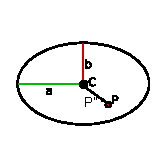
\includegraphics[scale=2]{sprint1/ellipse-collision}
	\caption{Vectors showing a point in the ellipse and the two radii.}
	\label{figure:ellipse-collision}
\end{figure}

\begin{equation}\label{eq:standard-equation}
	\frac{P_x^2}{a^2} + \frac{P_y^2}{b^2} \leq 1
\end{equation}

To use \formularef{eq:standard-equation}, we first have to accommodate for the rotation of the ellipse.
If the ellipse is rotated, we rotate the clicked point around the centre of the ellipse and compare it with an unrotated version of the ellipse.
The rotation of the clicked point is done by use of the rotation matrix, as seen in \formularef{eq:ellipses-rotation-matrix}.
An ellipse has two radii which are used in the formula and illustrated as $a$ and $b$, as seen in \figref{figure:ellipse-collision}.

\begin{equation}\label{eq:ellipses-rotation-matrix}
\begin{aligned}
	P'_x &= P''_x * cos(\alpha) - P''_y * sin(\alpha)\\
	P'_y &= P''_x * sin(\alpha) - P''_y * cos(\alpha)
\end{aligned}
\end{equation}

The variable $P''$ is the vector from the centre of the ellipse to the clicked point.
This formula can now replace the coordinate in the standard formula, which results in \formularef{eq:final-ellipses-equation}.

\begin{equation}\label{eq:final-ellipses-equation}
\begin{aligned}
	\frac{P_x^2}{a^2} &+ \frac{P_y^2}{b^2} \leq 1	\\
	&\Downarrow\\
	\frac{ P''_x * cos(\alpha) - P''_y * sin(\alpha)}{a^2} &+ \frac{P''_x * sin(\alpha) - P''_y * cos(\alpha)}{b^2} \leq 1\\
\end{aligned}
\end{equation}

With this final formula derived, we can use it in the program to check if the user has clicked on an ellipse or not.